\chapter{Load Cell Theoretical Response}

\section{Introduction}

Load cells are essential tools to measuring force in any industrial or
scientific system. One of the most common types of load cells is the strain
gauge load cell. In this type of load cell the deformation of a test material is
measured as a change in the electrical resistance of bonded strain gauge
elements. The test material that the load cell is made of is ideally very rigid,
otherwise significant elastic energy is stored by the load cell and it will
account for a non-negligible amount of deformation in the total system. Large
strains can also permanently damage the load cell by permanently deforming the
load cell or strain gauges and/or breaking the bonding of the load cells to
their substrate.

Here,  I will summarize the load cells used in the biaxial deformation apparatus
and provide a reference for calculations of the predicted load cell response and
calibration procedures. Calibration and verification of that calibration against
the predicted theoretical model is essential to performing accurate experiments
and ensuring that the system is performing as expected and not in need of
further maintenance/repair. 

\section{Load Cell Design}
Load cells on the biaxial apparatus are generally constructed of
beryllium-copper, but could be constructed of any material with the appropriate
properties. We desire a rigid material that can sustain several times the
maximum designed load without permanent deformation. Temperature stability is
the metal is also essential and resistive heating from the strain gauges and
environmental temperature changes can introduce undesirable zero point drift in
the system. Our design strives to cancel as much of these effects as possible.

\subsection{Material properties}
Our loads cells are made of Beryllium copper (BeCu). This material was chosen
for its resilience to repeated straining. It has long been a standard for
load cells and is a non-ferrous, non-sparking material. The material properties
are as follows in table 1.

\subsection{Mechanical design}
Currently we employ two load cell geometries: 1) a hollow ring with an
$\sim$62 mm outer diameter and $\sim$54 mm inner diameter, 2) a solid cylinder of $\sim$44 mm
diameter (Fig.\ref{load_cell_mechanical}). The load cells provide similar responses and are both linear with load under the applicable
conditions. The area of loading is important for modeling cell response. Area of the load cell can be 
calculated via eq.\ref{area} assuming a load cell outer diameter $r_o$ and inner diameter $r_i$.

% Equation %
\begin{equation}
	A = \pi(r_o^2-r_i^2)
	\label{area}
\end{equation}
% End Equation %

% Figure %
\begin{figure}
	\centering
		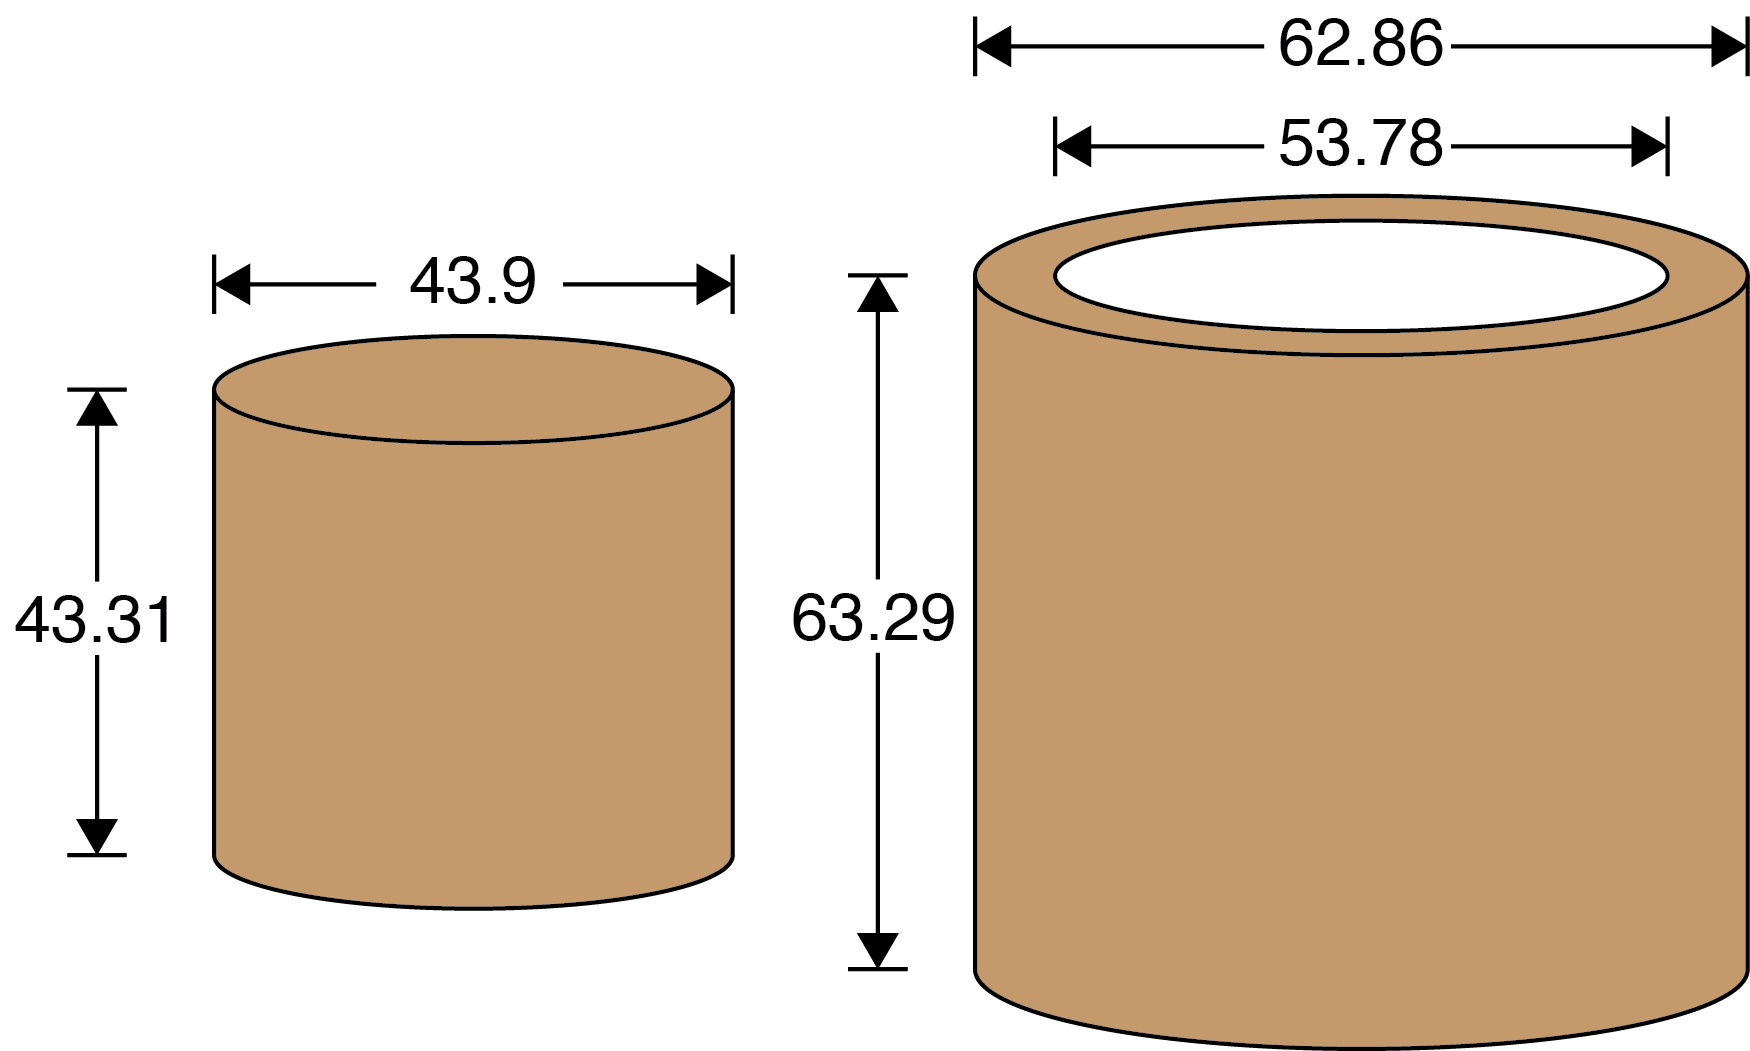
\includegraphics[scale=0.6]{appendix_load_response/load_cell_mechanical.png}
   	\caption{Mechanical drawings of the two styles of load cells used in the lab. Dimensions are in mm. Oblique view not to scale.}
  	\label{load_cell_mechanical}
\end{figure}
% End Figure %

\subsection{Electrical design}

Load cells are fitted with eight bonded foil strain gauges. This configuration provides high sensitivity and information from two orientations (axial and radial). A simple Wheatstone bridge configuration is used (Fig.\ref{load_cell_schematic}). Sets of gauges are placed at $90^\circ$ intervals around the load cell and bonded following the manufacturer's instructions. A cartoon of the construction and electrical hook-up is often helpful when troubleshooting or constructing load cells (Fig.\ref{load_cell_diagram}).  

% Figure %
\begin{figure}
	\centering
		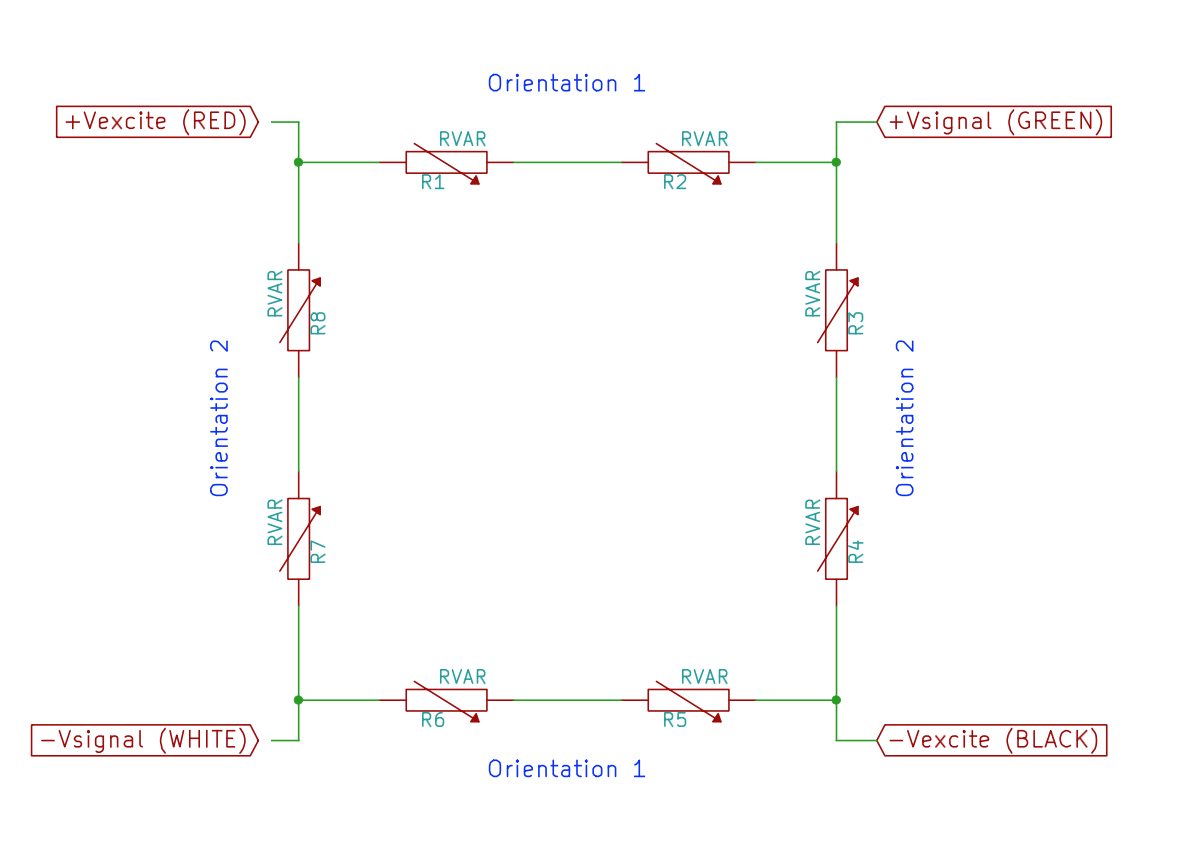
\includegraphics[scale=0.3]{appendix_load_response/load_cell_schematic.png}
   	\caption{Electrical schematic of the 8-gauge load cell design. Orientation 1 and 2 are marked for identification convenience.}
  	\label{load_cell_schematic}
\end{figure}
% End Figure %

% Figure %
\begin{figure}
	\centering
		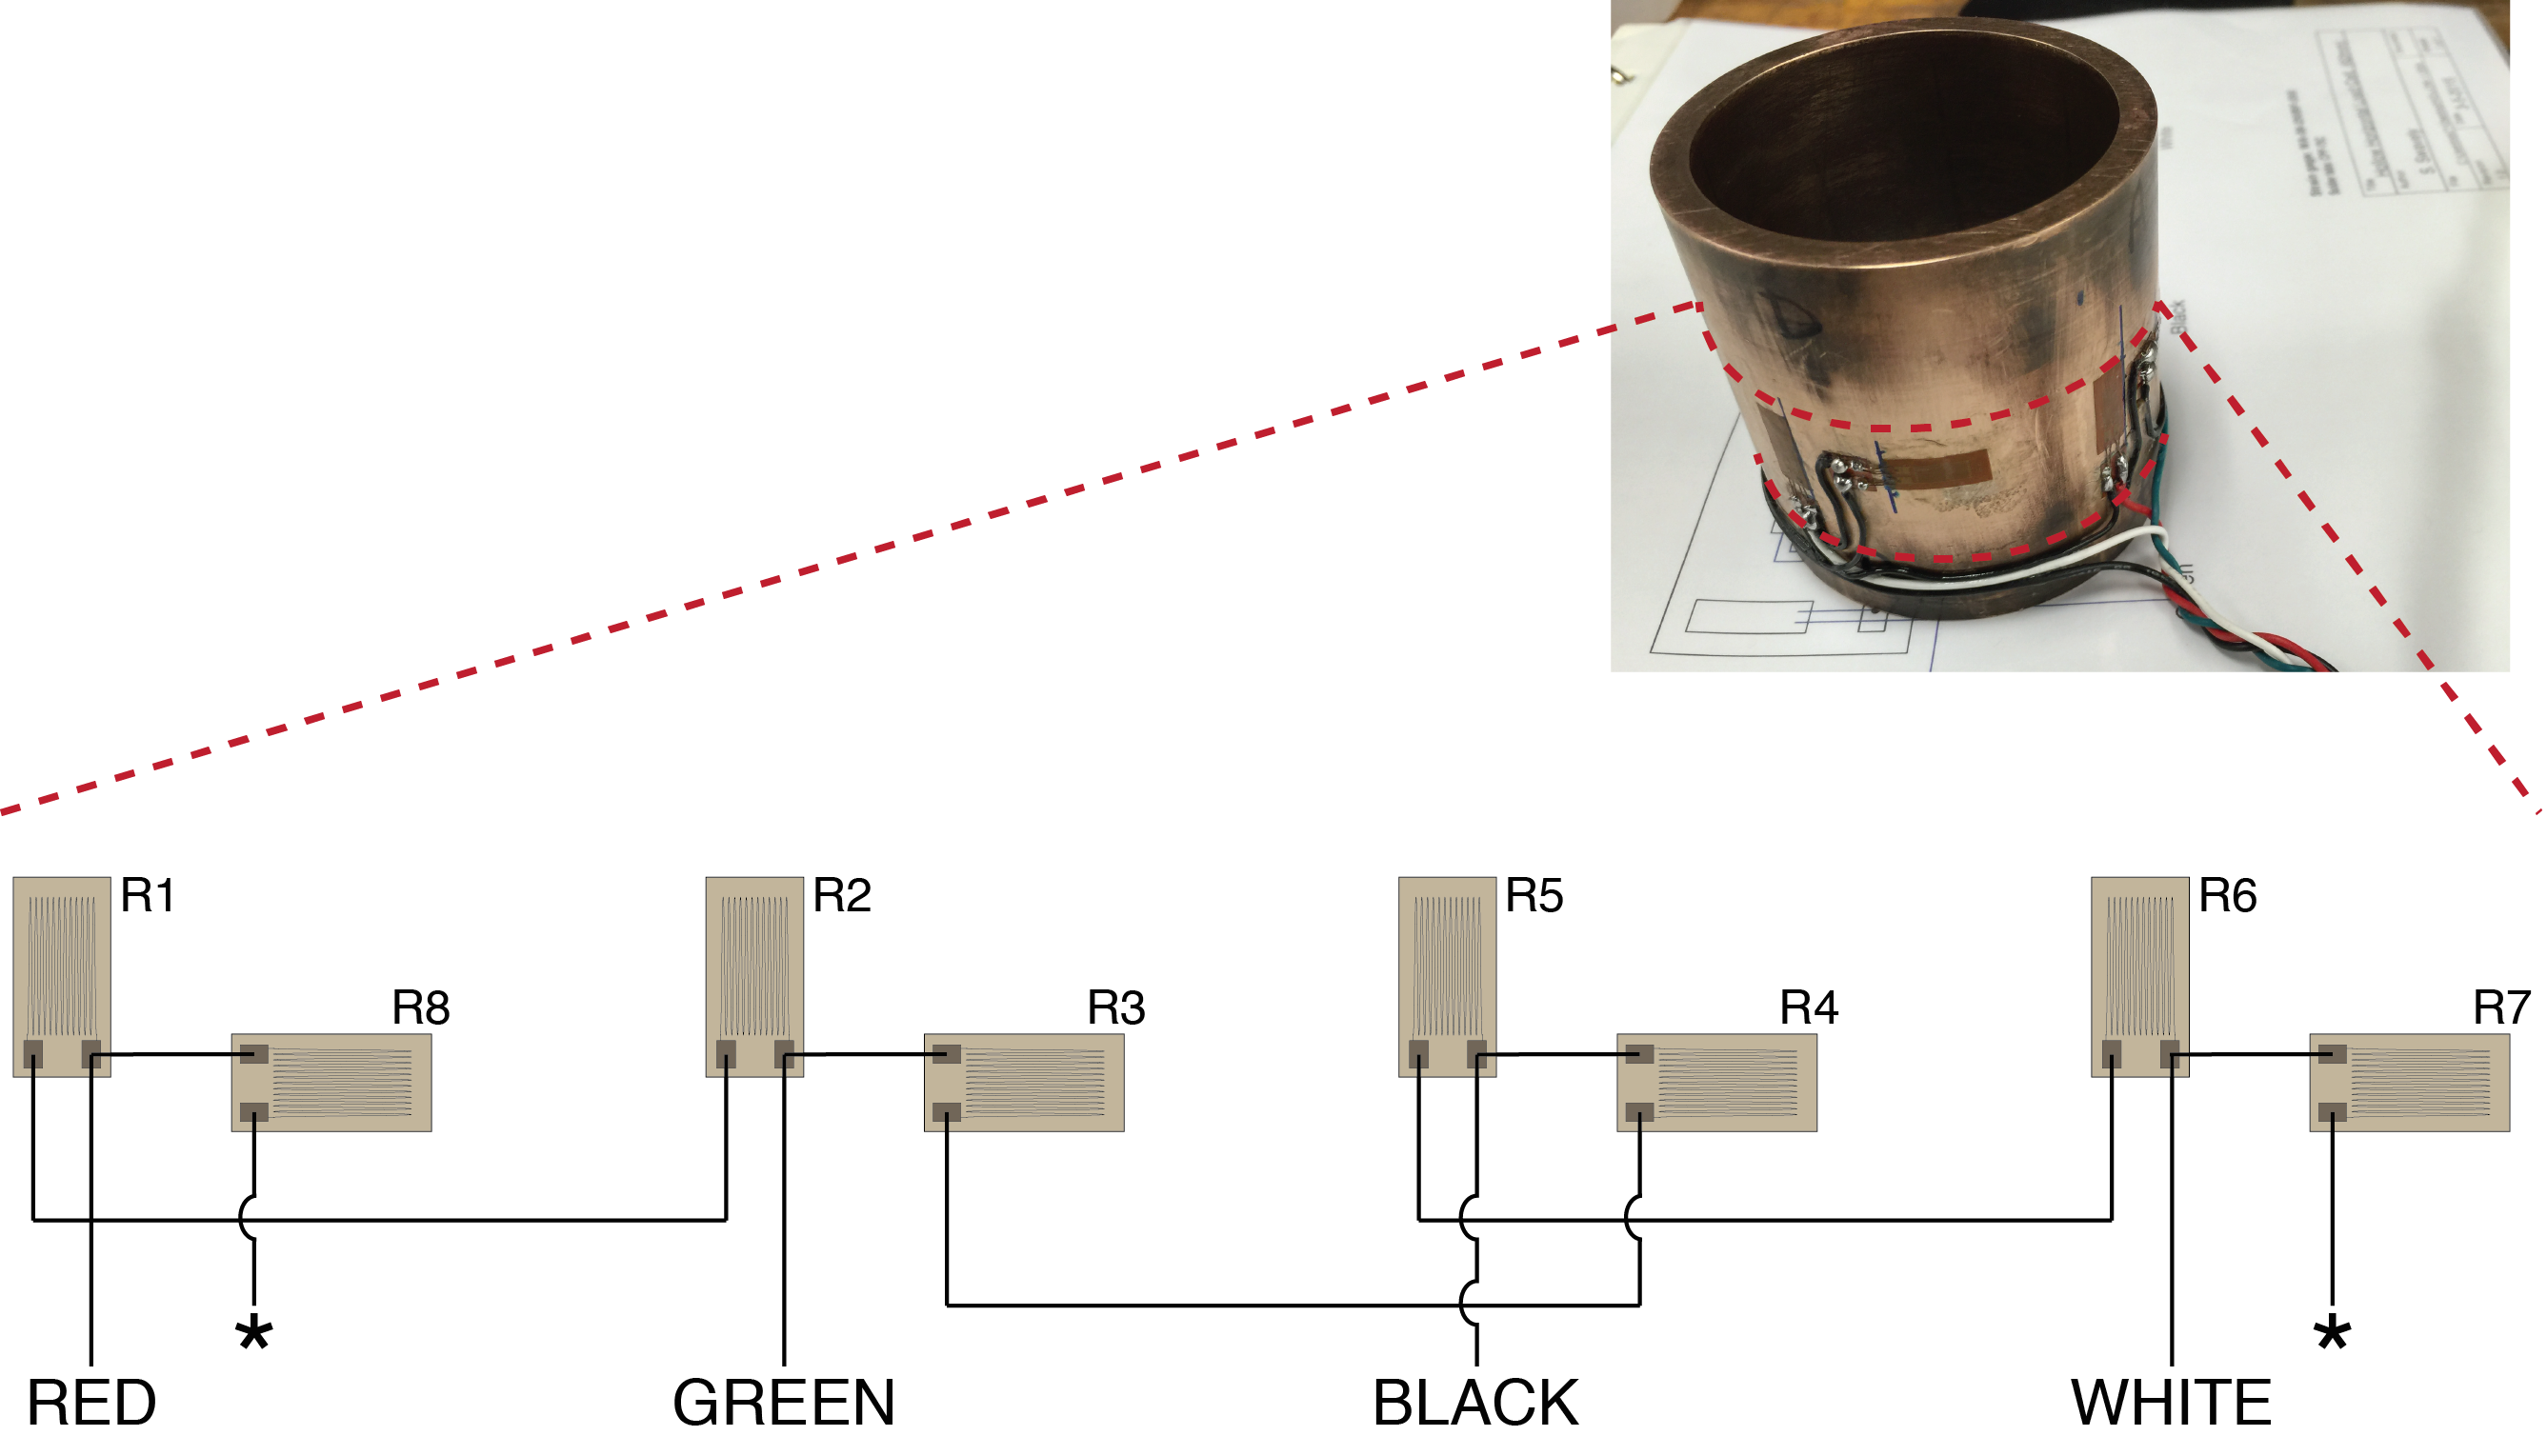
\includegraphics[scale=0.6]{appendix_load_response/load_cell.png}
   	\caption{Physical construction of the load cell and arrangement of strain gauges. gauge sets are set apart by $90^\circ$. Electrical points marked * are connected.}
  	\label{load_cell_diagram}
\end{figure}
% End Figure %

The Wheatstone bridge is excited by XX VDC provided by the strain gauge signal conditioner. The signal conditioner is a 1B31AN, manufactured by Analog Devices. A raw voltage from the load cell returns to the control system though an INA105 amplifier with switchable gain on the control panel (for the horizontal axis). The signal then passes to the 1B31AN for further gain and filtering.  

\section{Predicted response}

Predicting the response of the load cell involves calculating the mechanical response to stress and then transferring that information to calculations about the response of the strain gauges and amplifier circuits. This has been accomplished in a jupyter notebook that can be easily modified and experimented with. Here I will outline the basic procedure for the calcualtions.

First we must asertain the necessary mechanical properties of the load cell material. In this particular case, the shear modulus $(G)$ and Young's modulus $(E)$ were most easily obtained. Lame's first parameter can then be calculated using eq.\ref{lame}. With the elastic parameters in place, the response of the load cell to applied stress can be calculated. Since for the stresses applied in the lab BeCu behaves in a linear-elastic fashion, Hook's Law for elastic solids can be applied (eqs. \ref{hooke1},\ref{hooke2},\ref{hooke3}). These equations can be simplified for a case of uni-axial loading, but have been left in their full form to provide the most versatility for future application. Proof of equality is provided in the notebook. Initially intuition will say that a correction is needed for circumferential gauges, but writing out the equation for circumferential strain (eq.\ref{circ}) shows that no correction is needed since the diametric strain is equal to $\epsilon_3, \epsilon_3$.

% Equation %
\begin{equation}
	\lambda = \frac{G(E-2G)}{3G-E}
	\label{lame}
\end{equation}
% End Equation %

% Equation %
\begin{equation}
	\epsilon_1 = \sigma_1\frac{(\lambda+G)}{G(3 \lambda+2G)} - \sigma_2\frac{\lambda}{2G(3\lambda+2G)} -
\sigma_3\frac{\lambda}{2G(3\lambda+2G)}
	\label{hooke1}
\end{equation}
% End Equation %

% Equation %
\begin{equation}
	\epsilon_2 = -\sigma_1\frac{\lambda}{2G(3\lambda+2G)} + \sigma_2\frac{(\lambda+G)}{G(3 \lambda+2G)} - \sigma_3\frac{\lambda}{2G(3\lambda+2G)}
	\label{hooke2}
\end{equation}
% End Equation %

% Equation %
\begin{equation}
	\epsilon_3 = -\sigma_1\frac{\lambda}{2G(3\lambda+2G)} - \sigma_2\frac{\lambda}{2G(3\lambda+2G)} +
\sigma_3\frac{(\lambda+G)}{G(3 \lambda+2G)}
	\label{hooke3}
\end{equation}
% End Equation %

% Equation %
\begin{equation}
	\epsilon_c = \frac{\Delta c}{c_i} = \frac{\pi(d_f-d_i)}{\pi d_i}
	\label{circ}
\end{equation}
% End Equation %

Next the response of the strain gauges must be calculated. The fractional change in resistance per strain is characterized by the gauge factor $(\xi)$ of the particular strain gauge. This is a number typically near 2 for the strain gauges used in our applications. With slight manipulation the proportional resistance change to the no-strain resistance $(R_g)$ or the change is resistance is obtained through equation \ref{gauge_factor}. 


% Equation %
\begin{equation}
	\xi = \frac{\Delta R/R_g}{\epsilon}
	\label{gauge_factor}
\end{equation}
% End Equation %

With a predicted resistance change for each gauge, it is possible to calculate the bridge balance with equation \ref{bridge}. 

% Equation %
\begin{equation}
	V_{bridge} = V_{ex} \left(\frac{R_5 + R_6}{R_5 + R_6 + R_7 + R_8} - \frac{R_3 + R_4}{R_1 + R_2 + R_3 + R_4}\right)
	\label{bridge}
\end{equation}
% End Equation %
